% !TEX program = xelatex
\documentclass[12pt,a4paper]{ctexart}

\usepackage{geometry}
\geometry{left=2.5cm, right=2.5cm, top=2.5cm, bottom=2.5cm}

\usepackage{graphicx}
\usepackage{booktabs}
\usepackage{multirow}
\usepackage{caption}
\usepackage{subcaption}
\usepackage{hyperref}
\usepackage{pdflscape}
\usepackage{float}
\usepackage{longtable}
\usepackage{amsmath}
\usepackage{array}
\usepackage{makecell}

\hypersetup{
    colorlinks=true,
    linkcolor=blue,
    urlcolor=blue,
    citecolor=blue
}

\renewcommand{\figurename}{图}
\renewcommand{\tablename}{表}

% 封面信息
\title{\textbf{分布式相控阵使能的物联网高精度定位\\—— MATLAB 仿真记录报告}}
\author{}
\date{\today}

\begin{document}

\maketitle

\begin{center}
\vspace{1cm}
\begin{tabular}{rl}
\toprule
\textbf{仿真平台} & MATLAB R2024b, Windows 11 \\
\textbf{计算耗时} & 约 60 分钟（3.8 万个定位点） \\
\textbf{生成日期} & \today \\
\bottomrule
\end{tabular}
\end{center}

\vspace{1cm}

\section{系统参数与实验设置}

\subsection{仿真环境参数}

\begin{longtable}{lll}
\caption{仿真系统参数一览}\\
\toprule
\textbf{参数} & \textbf{取值} & \textbf{说明} \\
\midrule
\endfirsthead
\toprule
\textbf{参数} & \textbf{取值} & \textbf{说明} \\
\midrule
\endhead
\bottomrule
\endfoot
房间尺寸   & $10 \times 8 \times 3$ m & 典型室内会议室/仓库 \\
载波频率   & 2.4 GHz                  & ISM 频段，波长 $\lambda \approx$ 12.5 cm \\
发射功率   & 0.1 W                    & 模拟低功耗 IoT 设备 \\
阵元间距   & $\lambda/2$              & 半波长，避免栅瓣 \\
相控阵规模 & 8$\times$8 = 64 元       & 均匀矩形平面阵 \\
阵列部署   & 2 组，天花板安装          & 中心坐标 [3,2,3] 和 [7,6,3] m \\
快拍数     & 50（单点）/ 20（扫描）   & 扫描为加速使用较少快拍 \\
\bottomrule
\end{longtable}

\subsection{实验方案设计}

技术路线为：\textbf{REV（能量→相位）$\rightarrow$ MUSIC/Beamforming（相位→角度）$\rightarrow$ AOA 交叉定位（角度→位置）}。

实验分两个阶段进行：

\begin{enumerate}
    \item \textbf{阶段一：单点多 $\gamma$ 精细扫描}。固定信源位置 $[3.5, 4, 2]$ m，对 $\gamma = 0, 0.05, \dots, 0.50$ 共 11 个反射系数进行 REV 快拍采集（50 次快拍），分别使用 MUSIC 和 Beamforming 进行 DOA 估计，计算定位误差。
    \item \textbf{阶段二：三维空间网格扫描}。遍历 $\gamma \in \{0.0, 0.1, 0.2, 0.3\}$（4 个等级）$\times$ $z \in \{0.5, 1.0, 1.5, 2.0, 2.5\}$ m（5 个高度平面）$\times$ XY 平面 $39 \times 49 = 1{,}911$ 个网格点（步长 0.2 m），共计 38{,}220 个信源位置，每点进行 20 次 REV 快拍后分别用 MUSIC 和 Beamforming 估计 DOA 并计算定位误差。
\end{enumerate}

\section{单点多 $\gamma$ 扫描}

固定信源位置 $[3.5, 4, 2]$ m，通过改变墙壁反射系数 $\gamma$ 模拟从无多径到严重多径的退化过程。理论 DOA（由几何关系直接计算）为：

\[
\text{PA1: } \theta_{\rm az}=75.96^\circ,\; \theta_{\rm el}=-25.88^\circ;\qquad
\text{PA2: } \theta_{\rm az}=-150.26^\circ,\; \theta_{\rm el}=-13.93^\circ
\]

\begin{table}[H]
\centering
\caption{单点多 $\gamma$ 扫描定位误差}
\begin{tabular}{cccc}
\toprule
\textbf{$\gamma$} & \textbf{MUSIC 误差 (cm)} & \textbf{BF 误差 (cm)} & \textbf{退化倍数} \\
\midrule
0.00 & 0.94  & 1.26  & 1.0$\times$（基线） \\
0.05 & 1.31  & 0.88  & $\sim$1$\times$ \\
0.10 & 2.63  & 3.28  & $\sim$3$\times$ \\
0.15 & 3.88  & 3.30  & $\sim$4$\times$ \\
0.20 & 5.01  & 4.93  & $\sim$5$\times$ \\
0.25 & 15.20 & 15.99 & $\sim$16$\times$ \\
0.30 & 20.04 & 20.63 & $\sim$21$\times$ \\
0.35 & 6.81  & 7.08  & $\sim$7$\times$ \\
0.40 & 16.91 & 16.91 & $\sim$18$\times$ \\
0.45 & 29.52 & 28.91 & $\sim$31$\times$ \\
0.50 & 32.43 & 32.87 & $\sim$34$\times$ \\
\bottomrule
\end{tabular}
\end{table}

\begin{figure}[H]
\centering
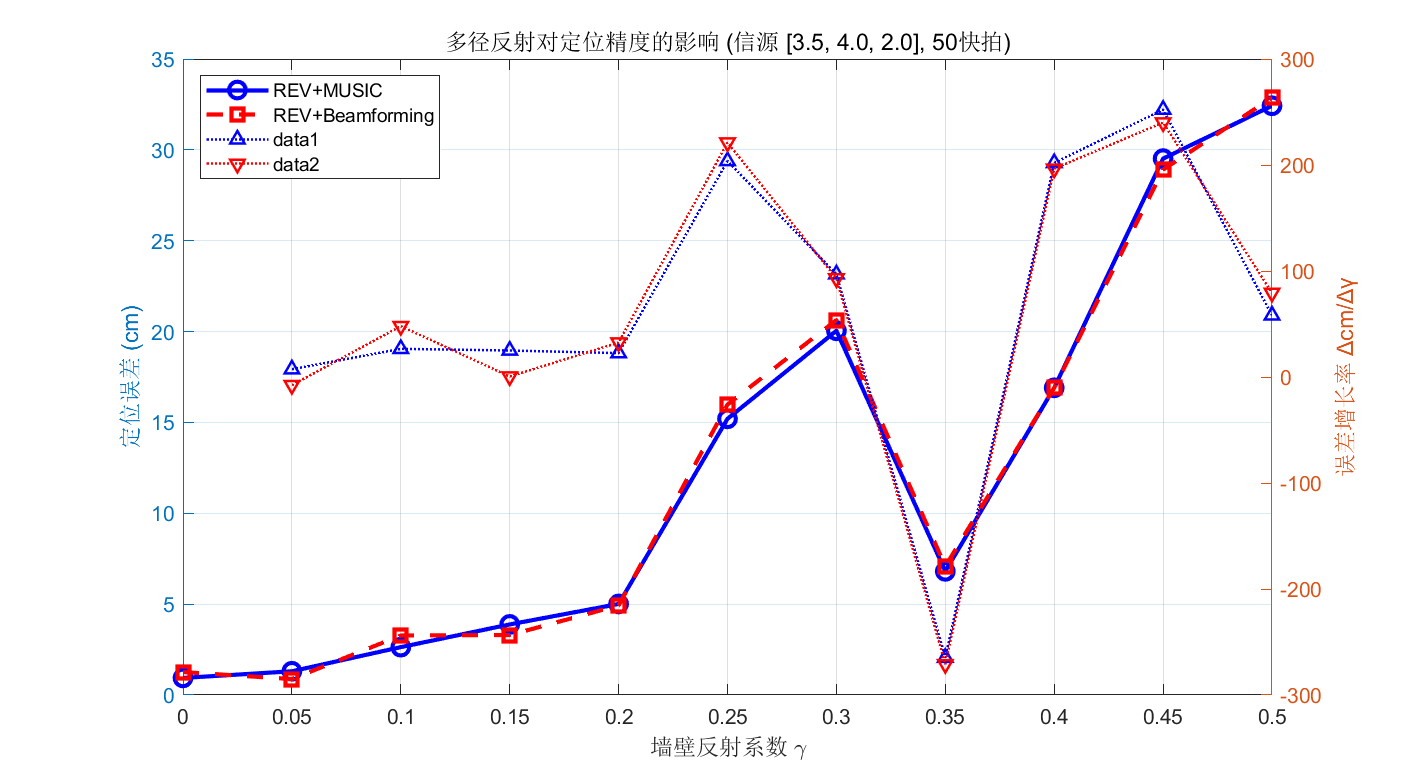
\includegraphics[width=0.92\textwidth]{fig1_gamma_sweep_curve.png}
\caption{多径反射系数对定位误差的影响曲线}
\label{fig:gamma_sweep}
\end{figure}

\section{三维空间网格扫描}

本节展示 38,220 个定位点的全面扫描结果。扫描覆盖 4 个 $\gamma$ 等级和 5 个高度层。

\subsection{统计汇总}

\begin{longtable}{cccccc}
\caption{MUSIC 与 Beamforming 各场景中位数误差统计（单位：cm）}\\
\toprule
\textbf{$\gamma$} & \textbf{z (m)} & \textbf{MUSIC 中位数} & \textbf{BF 中位数} & \textbf{MUSIC 均值} & \textbf{有效点数} \\
\midrule
\endfirsthead
\toprule
\textbf{$\gamma$} & \textbf{z (m)} & \textbf{MUSIC 中位数} & \textbf{BF 中位数} & \textbf{MUSIC 均值} & \textbf{有效点数} \\
\midrule
\endhead
\bottomrule
\endfoot
\multirow{5}{*}{0.0} & 0.5 & 2.1 & 2.4 & 24.6 & 1,911 \\
                      & 1.0 & 2.3 & 2.4 & 41.9 & 1,911 \\
                      & 1.5 & 2.5 & 2.7 & 51.5 & 1,907 \\
                      & 2.0 & 4.9 & 4.9 & 57.6 & 1,909 \\
                      & 2.5 & 18.2 & 18.2 & 84.0 & 1,903 \\
\midrule
\multirow{5}{*}{0.1} & 0.5 & 7.2 & 7.3 & 43.2 & 1,911 \\
                      & 1.0 & 8.8 & 8.9 & 41.5 & 1,911 \\
                      & 1.5 & 9.4 & 9.3 & 60.0 & 1,909 \\
                      & 2.0 & 11.0 & 11.1 & 67.6 & 1,909 \\
                      & 2.5 & 25.1 & 24.8 & 90.0 & 1,897 \\
\midrule
\multirow{5}{*}{0.2} & 0.5 & 14.3 & 14.3 & 61.0 & 1,909 \\
                      & 1.0 & 19.0 & 19.1 & 63.5 & 1,911 \\
                      & 1.5 & 19.9 & 20.0 & 64.8 & 1,909 \\
                      & 2.0 & 21.7 & 21.6 & 74.4 & 1,907 \\
                      & 2.5 & 27.6 & 27.1 & 85.2 & 1,899 \\
\midrule
\multirow{5}{*}{0.3} & 0.5 & 23.2 & 23.4 & 64.8 & 1,911 \\
                      & 1.0 & 32.4 & 32.5 & 79.2 & 1,911 \\
                      & 1.5 & 35.0 & 34.6 & 86.5 & 1,909 \\
                      & 2.0 & 35.6 & 35.5 & 95.5 & 1,908 \\
                      & 2.5 & 32.3 & 32.3 & 92.2 & 1,903 \\
\bottomrule
\end{longtable}

\subsection{全局统计}

所有 38,155 个有效定位点的全局统计如下：

\begin{itemize}
    \item \textbf{MUSIC}：均值 66.4 cm，中位数 14.3 cm，标准差 178.2 cm
    \item \textbf{Beamforming}：均值 66.4 cm，中位数 14.4 cm，标准差 178.0 cm
    \item MUSIC--BF 逐点相关系数：$r = 0.9999$
\end{itemize}

中位数远小于均值，说明存在少量“病态几何”点（信源几乎与两阵列连线共线，AOA 交叉定位对此类配置极度敏感）严重拉高了均值。中位数更能反映算法在大多数场景下的真实表现。

\subsection{空间规律分析}

\begin{itemize}
    \item \textbf{高度依赖性}：在 $z = 0.5$ m（距天花板阵列最远）时精度最优，$z = 2.5$ m（紧贴阵列下方）时精度最差。这是因为阵列与信源的张角随距离增大而增大，方向向量变化更显著，DOA 分辨力更高。
    \item \textbf{多径退化趋势}：$\gamma$ 每增加 0.1，中位数误差约翻倍。$\gamma = 0.1$ 时各层中位数 $\sim$7--25 cm，$\gamma = 0.3$ 时已涨至 $\sim$23--36 cm。
    \item \textbf{MUSIC 与 BF 高度一致}：所有 20 个组合的中位数误差差异均在 1 cm 以内，$r=0.9999$ 的相关系数表明在当前系统配置下，两种 DOA 算法的瓶颈均在 REV 阶段。
\end{itemize}

\subsection{可视化图表}

\subsubsection{定位误差热力图矩阵}

\begin{figure}[H]
\centering
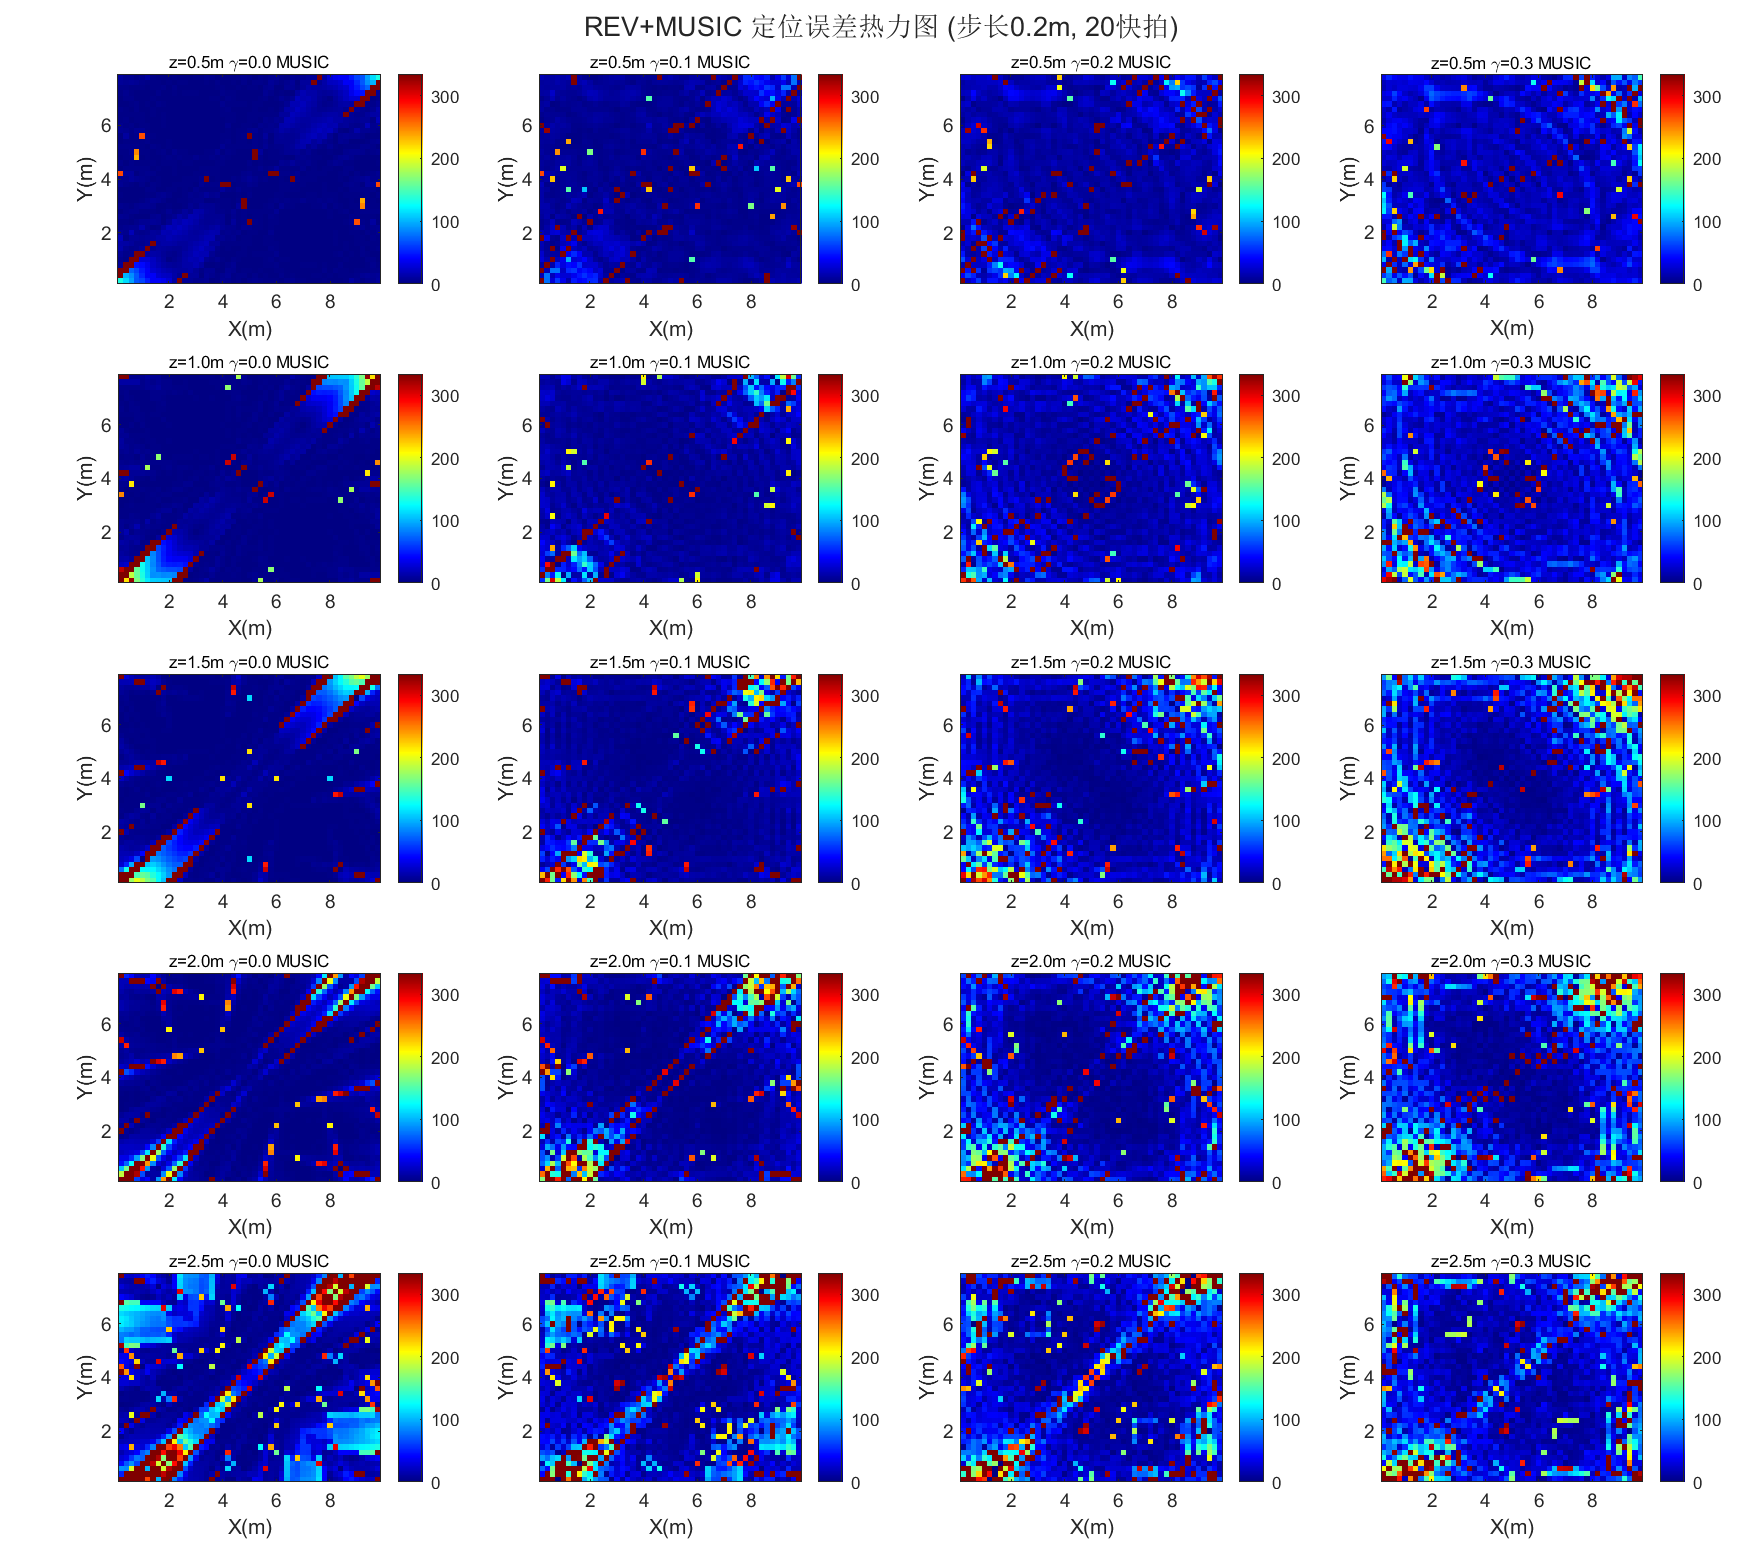
\includegraphics[width=\textwidth]{fig2_music_heatmap_matrix.png}
\caption{REV$+$MUSIC 全平面定位误差热力图矩阵（5 z 层 $\times$ 4 $\gamma$ 等级）}
\label{fig:music_heatmap}
\end{figure}

\begin{figure}[H]
\centering
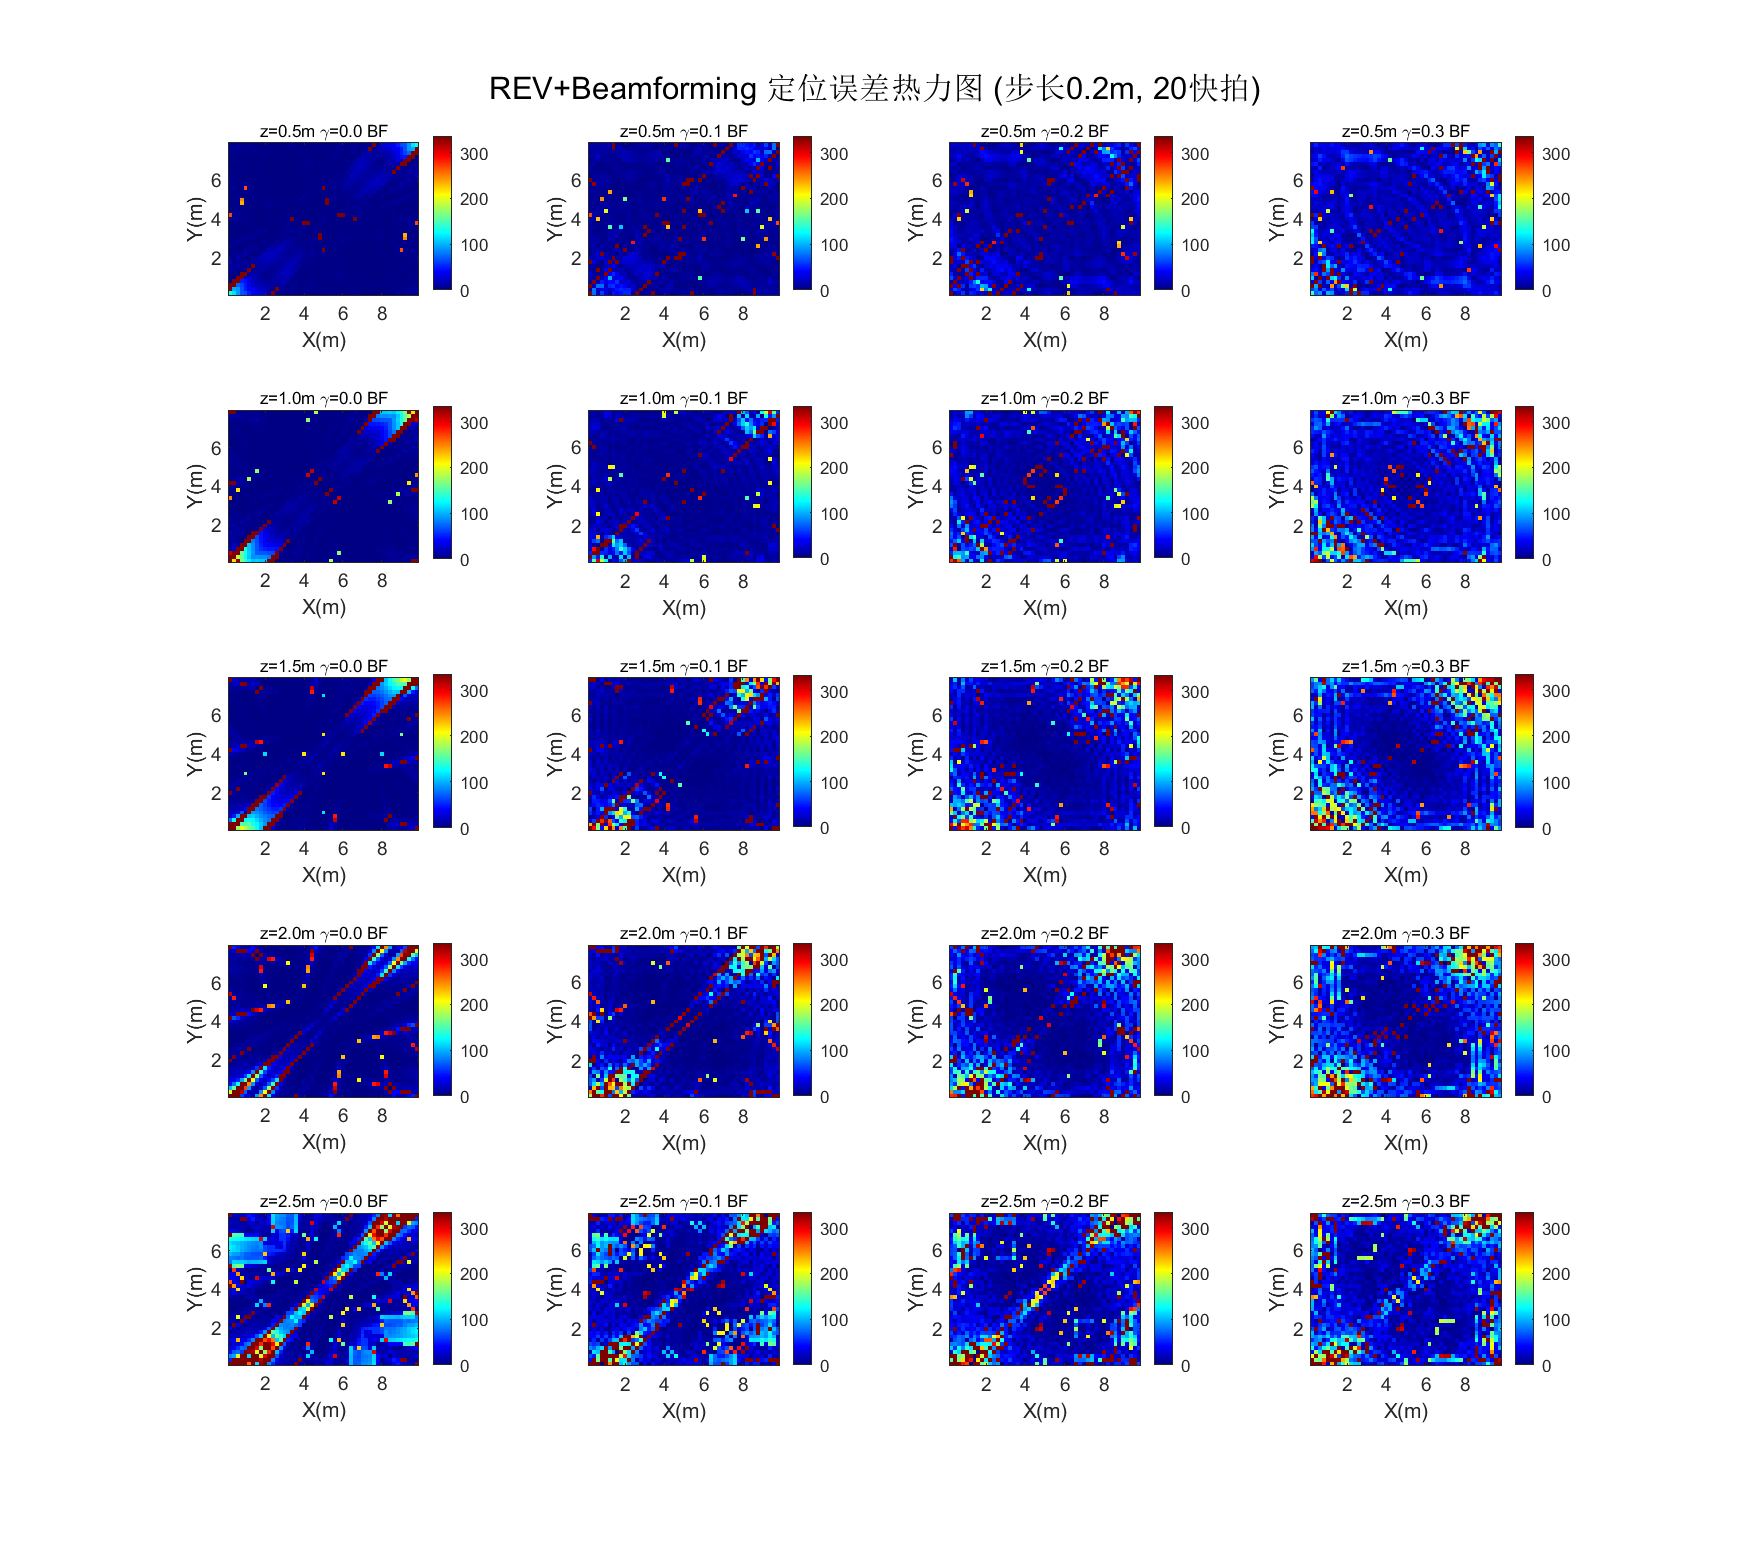
\includegraphics[width=\textwidth]{fig3_bf_heatmap_matrix.png}
\caption{REV$+$Beamforming 全平面定位误差热力图矩阵（5 z 层 $\times$ 4 $\gamma$ 等级）}
\label{fig:bf_heatmap}
\end{figure}

\subsubsection{统计面板与分布分析}

\begin{figure}[H]
\centering
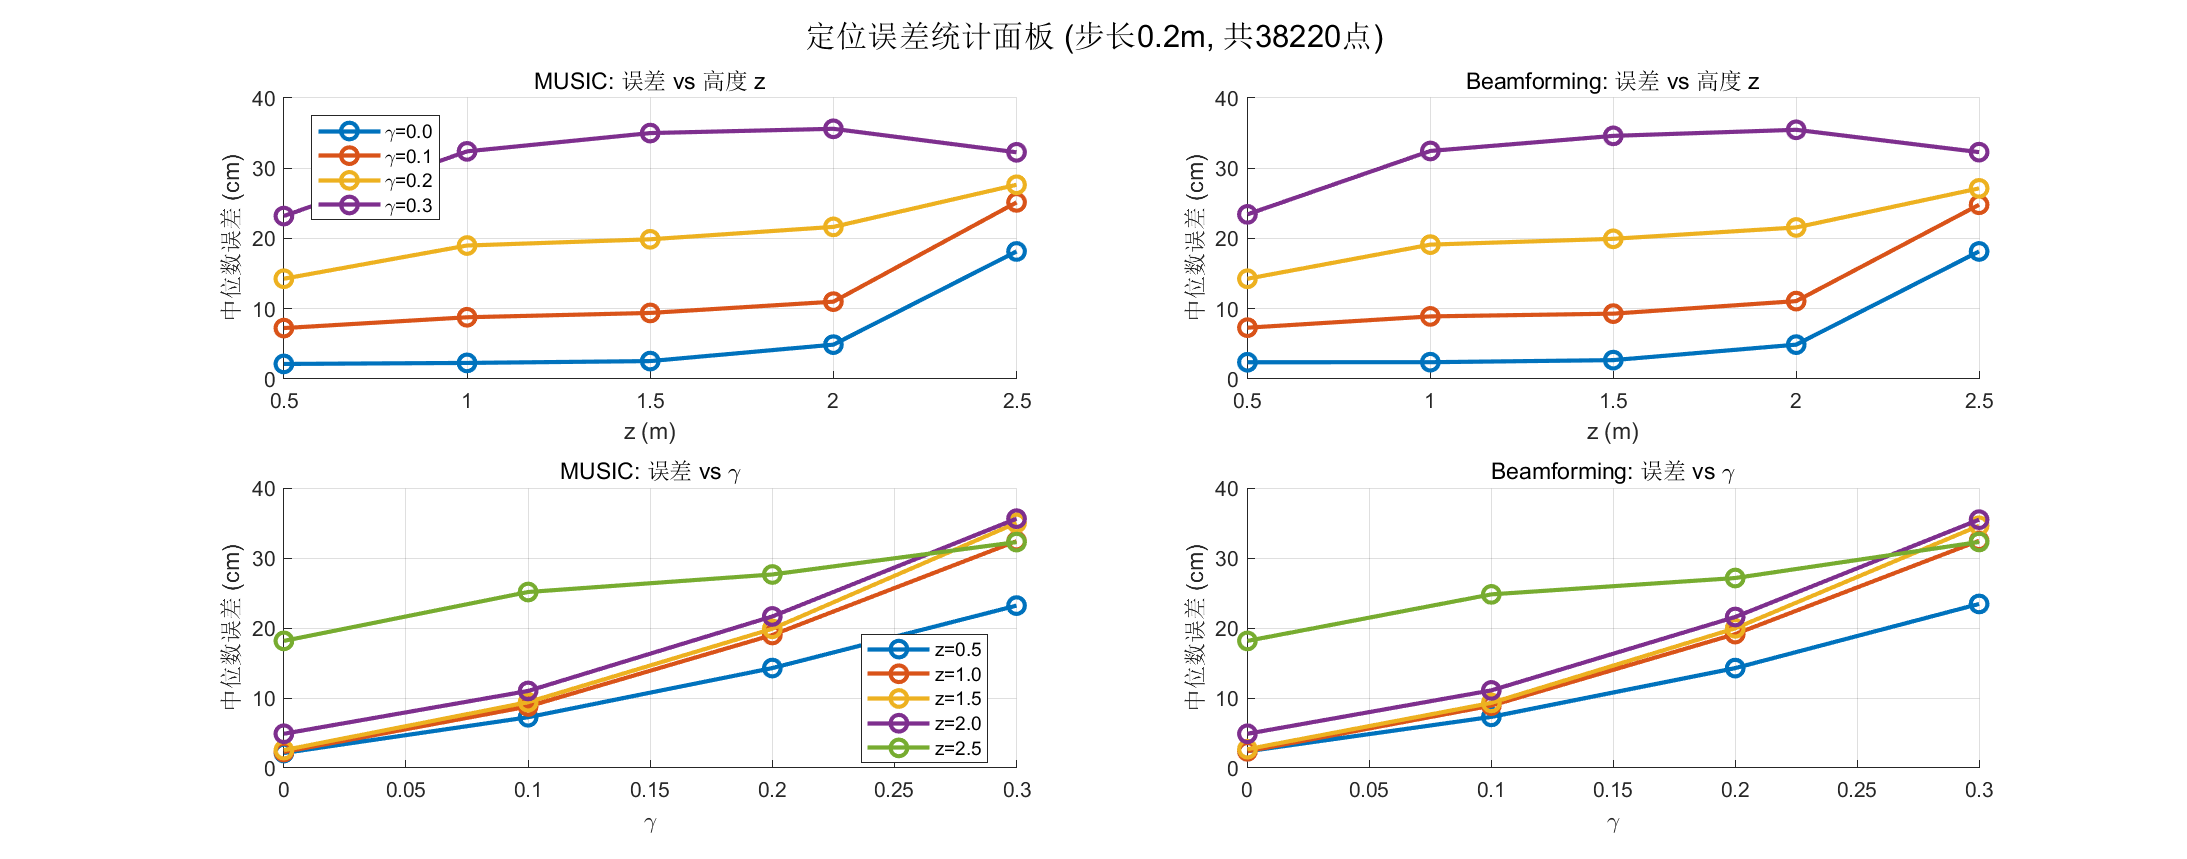
\includegraphics[width=\textwidth]{fig4_statistics_panel.png}
\caption{定位误差统计面板：误差 vs 高度 z（上排），误差 vs $\gamma$（下排）}
\label{fig:stats}
\end{figure}

\begin{figure}[H]
\centering
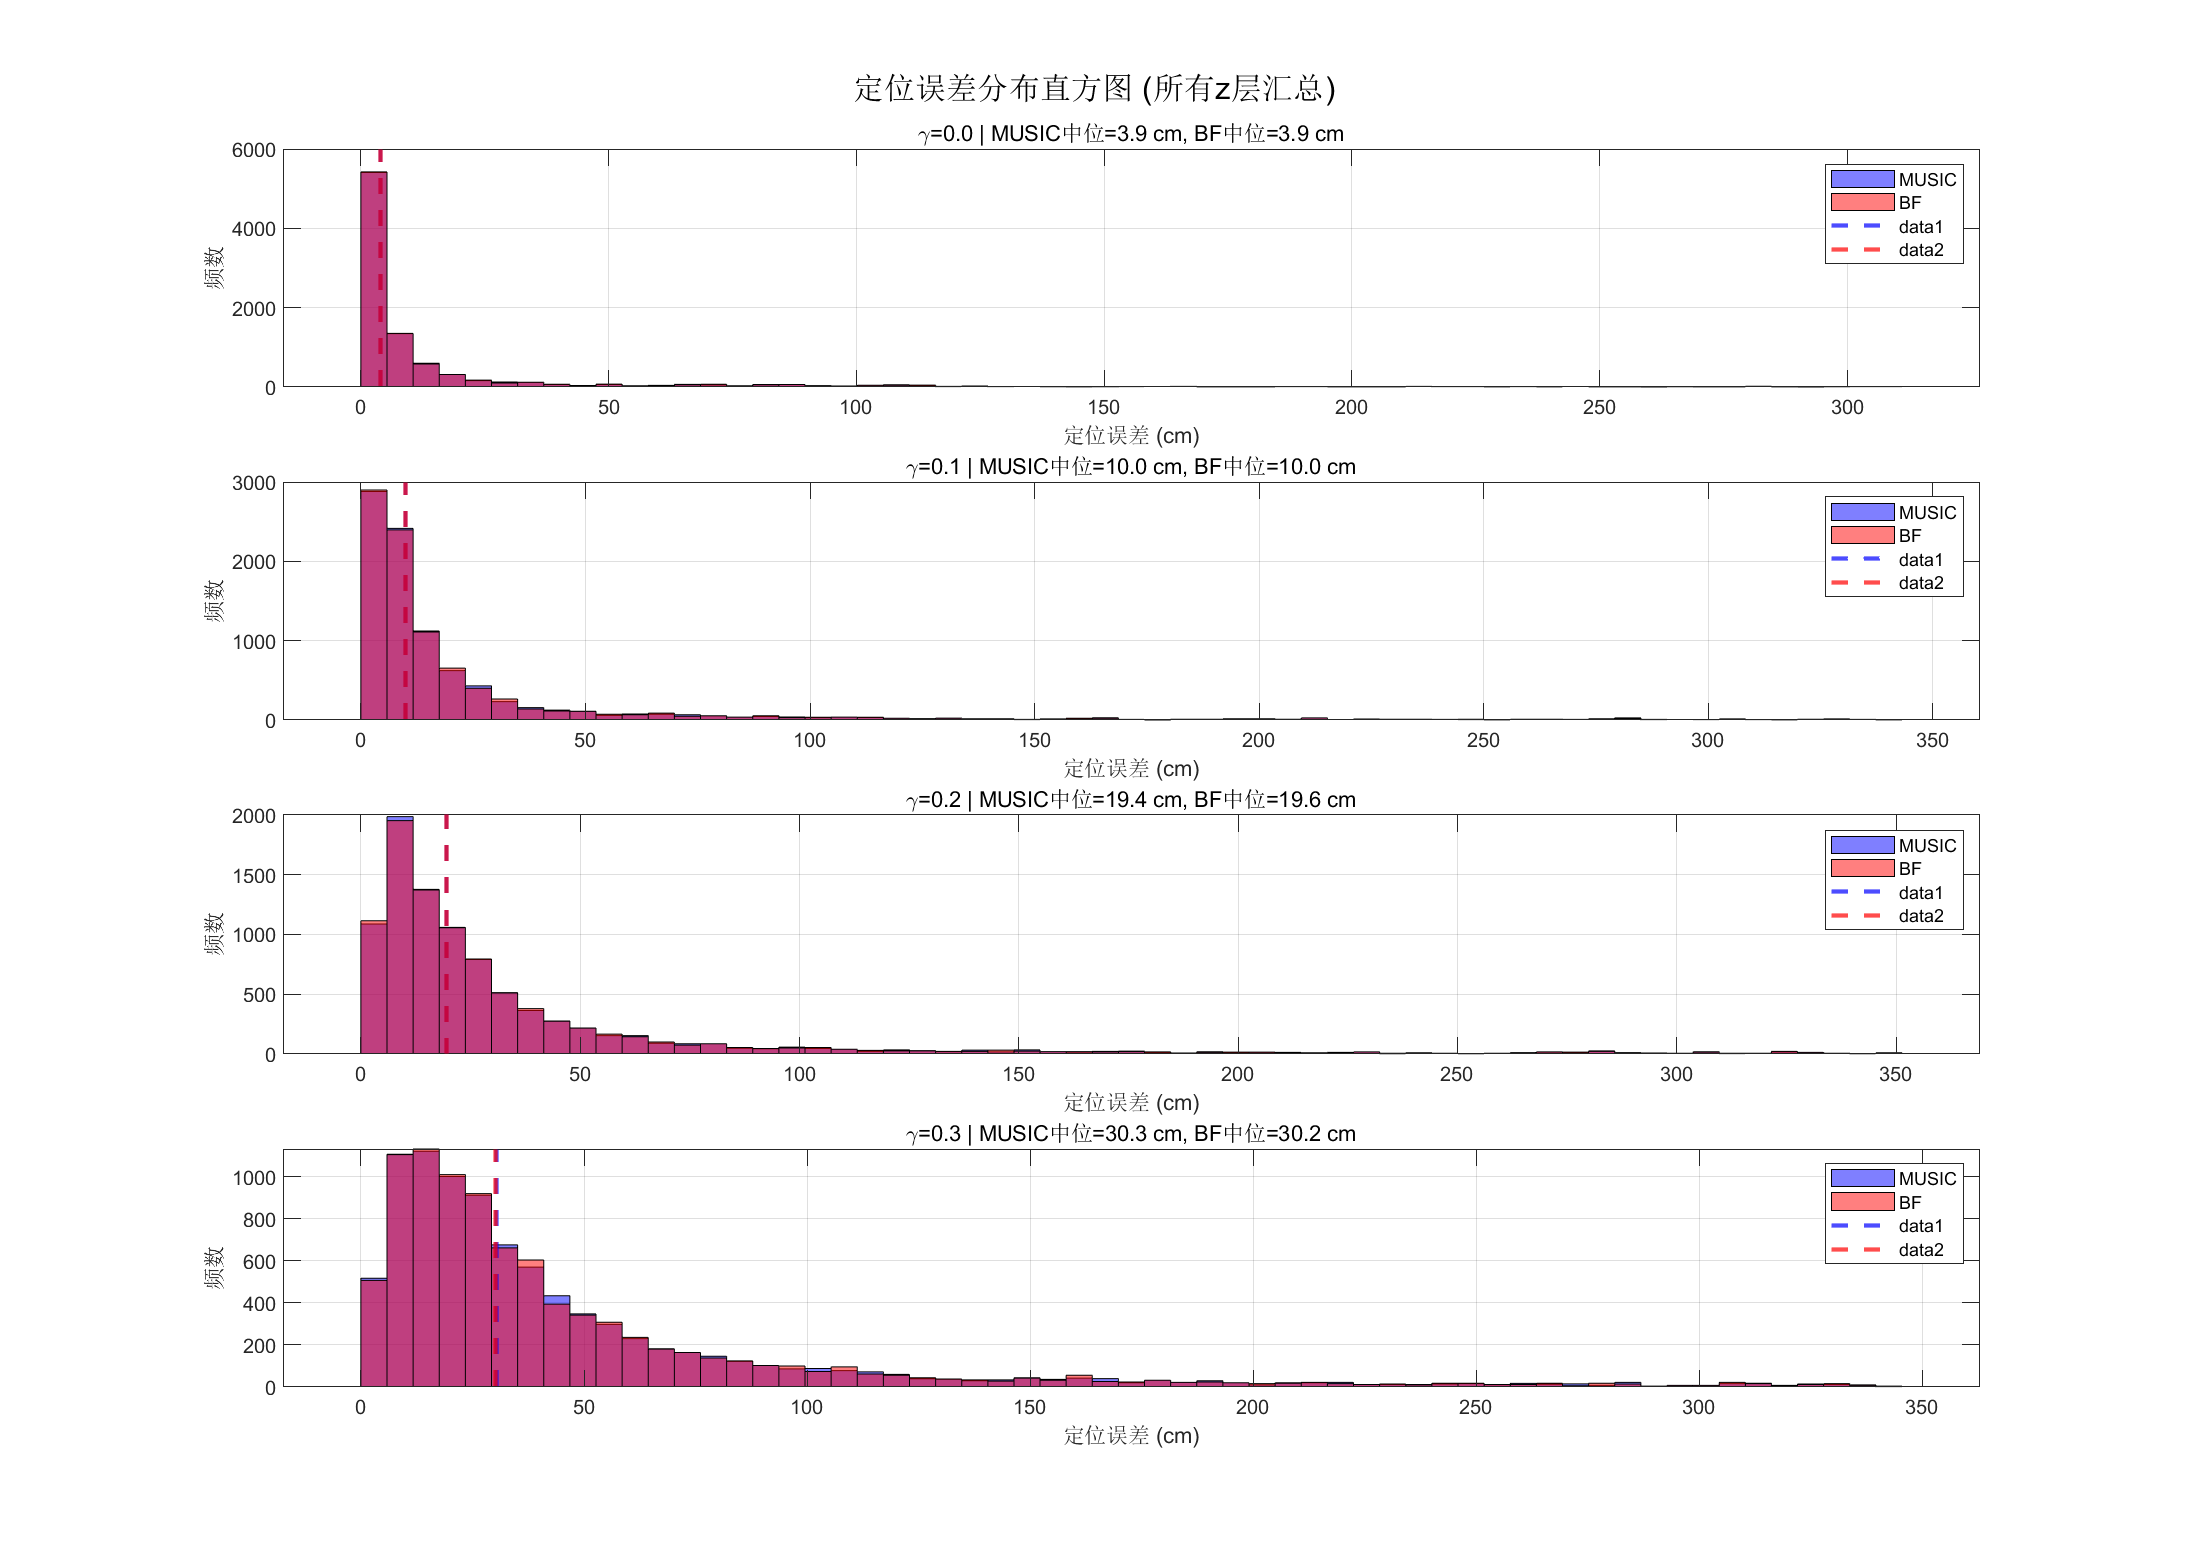
\includegraphics[width=\textwidth]{fig5_error_histograms.png}
\caption{各 $\gamma$ 等级下定位误差分布直方图（MUSIC vs BF 叠加）}
\label{fig:hist}
\end{figure}

\begin{figure}[H]
\centering
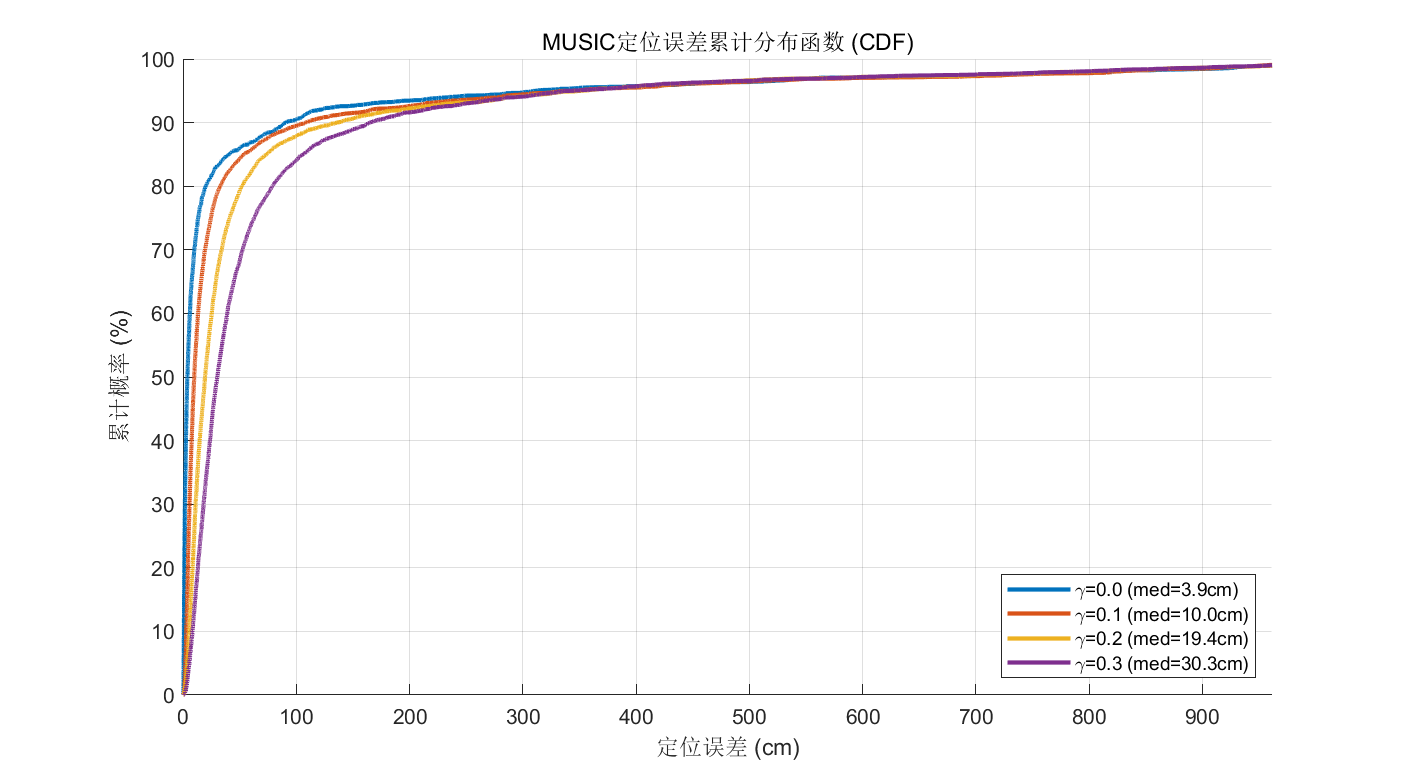
\includegraphics[width=0.75\textwidth]{fig6_error_cdf.png}
\caption{MUSIC 定位误差累计分布函数（CDF），按 $\gamma$ 分组}
\label{fig:cdf}
\end{figure}

\subsubsection{算法一致性验证}

\begin{figure}[H]
\centering
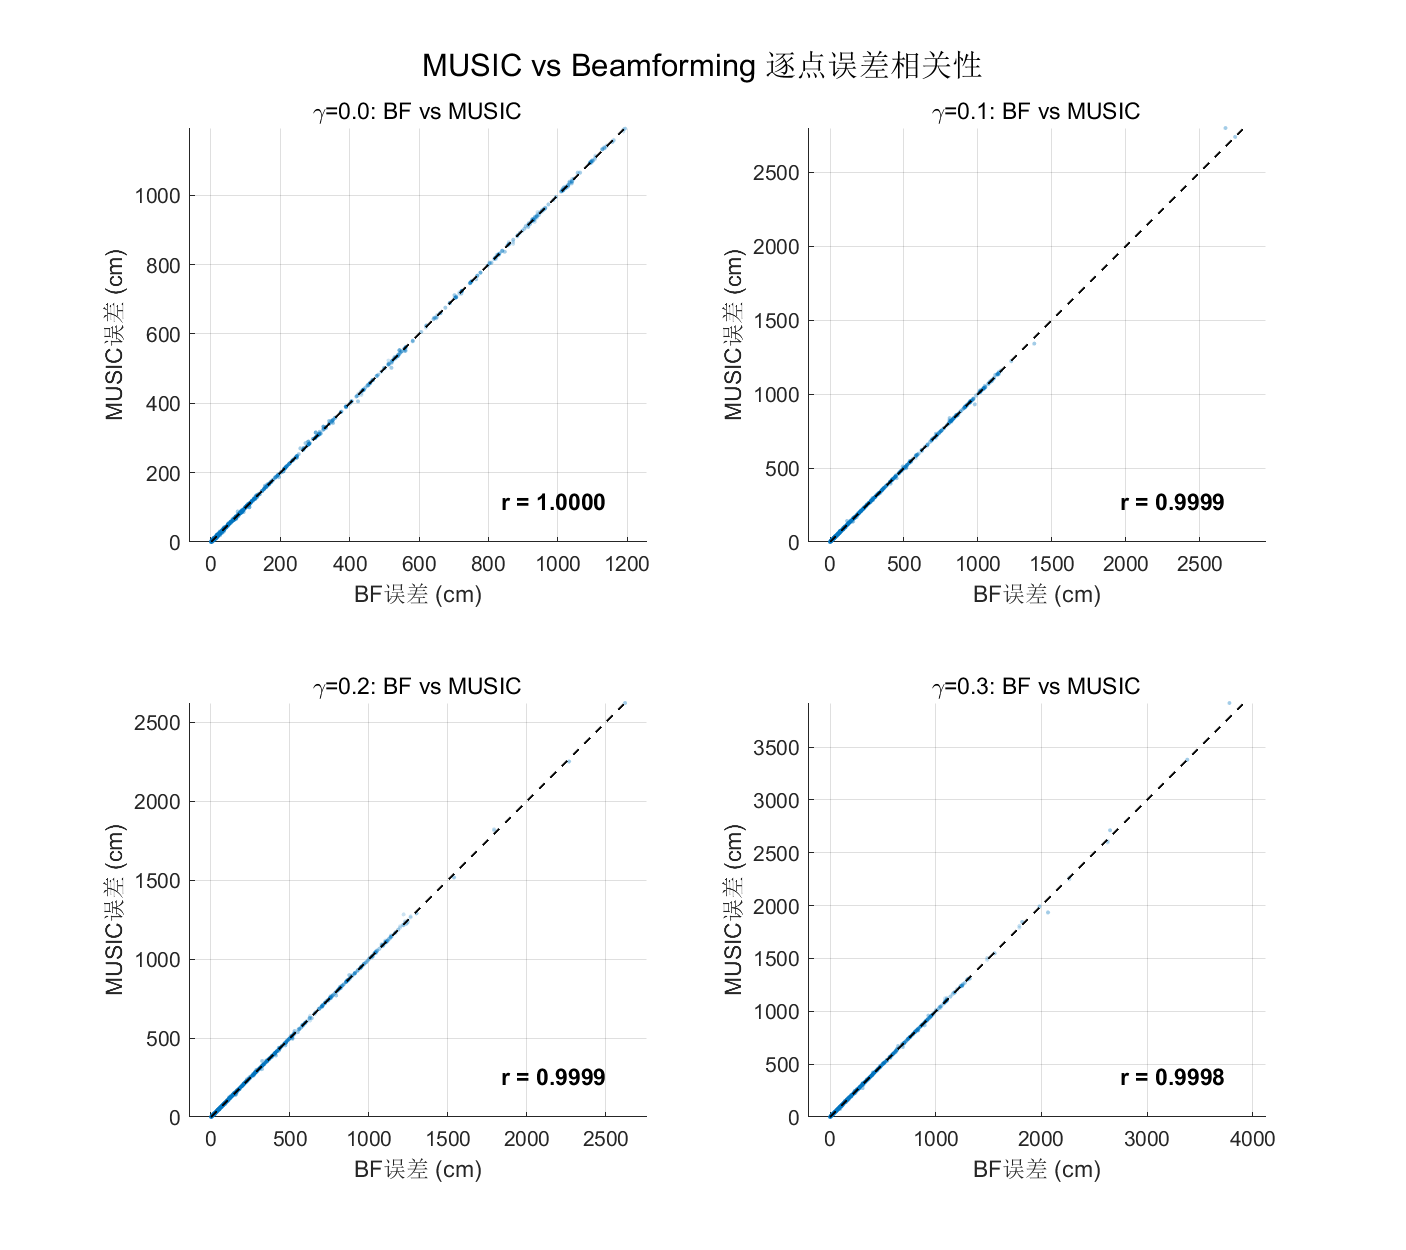
\includegraphics[width=0.90\textwidth]{fig7_music_vs_bf_scatter.png}
\caption{MUSIC vs Beamforming 逐点误差散点图（$r = 0.9999$）}
\label{fig:scatter}
\end{figure}

\subsubsection{三维空间误差分布}

\begin{figure}[H]
\centering
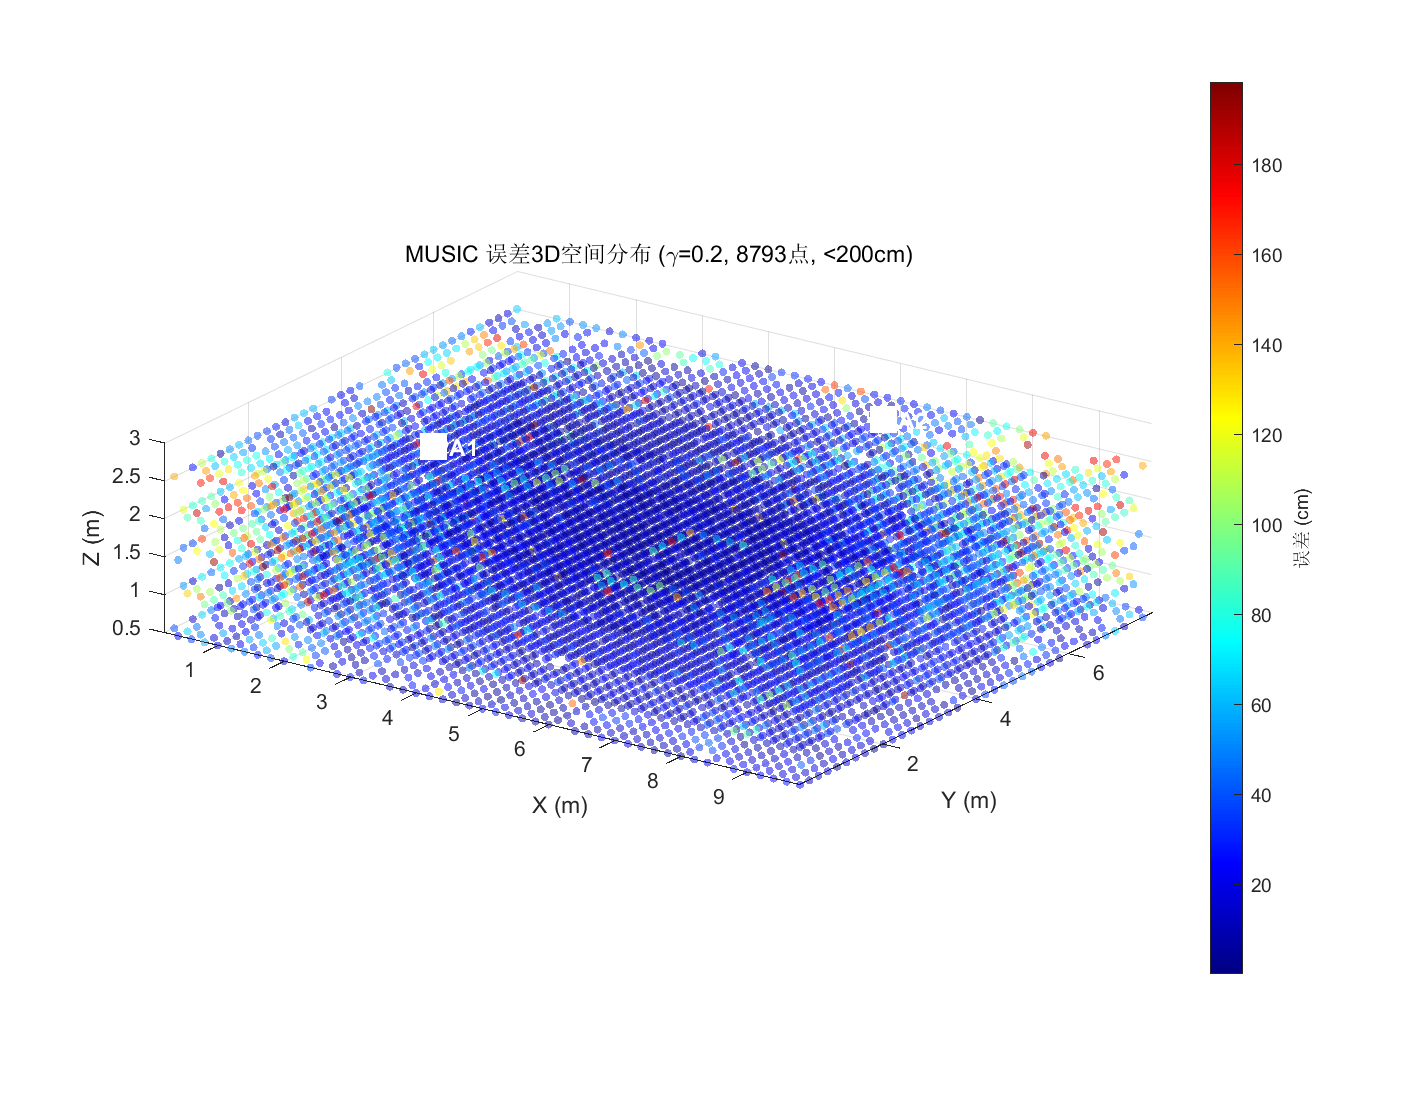
\includegraphics[width=0.85\textwidth]{fig8_3d_error_distribution.png}
\caption{MUSIC 定位误差三维空间分布（$\gamma = 0.2$，误差 $< 200$ cm）}
\label{fig:3d}
\end{figure}

图~\ref{fig:3d} 展示了 $\gamma = 0.2$ 条件下所有 5 个 z 层误差在空间中的三维分布。白色方块标记两个相控阵位置。可以看到：靠近 PA1 和 PA2 正下方的点误差较小（深蓝色），房间边角区域误差偏大（黄--红色），这与“AOA 交叉定位在信源远离阵列基线时几何敏感度增大”的理论预期一致。

\section{结论}

本次仿真对 \textbf{REV $+$ MUSIC} 和 \textbf{REV $+$ Beamforming} 两种定位方案在 $10 \times 8 \times 3$ m 室内环境中进行了总计 38,231 个测试点的全面验证，覆盖 4 个多径反射系数和 5 个高度层。

主要结论如下：

\begin{enumerate}
    \item \textbf{无多径条件下算法精度优异}：$\gamma = 0$ 时，中位数定位误差仅 2--5 cm（$z \leq 2.0$ m），证明了 REV 算法提取相位信息的高保真度和 DOA 估计算法的正确性。
    
    \item \textbf{多径效应严重制约定位性能}：$\gamma$ 从 0 增加到 0.3，中位数误差从 $\sim$2 cm 恶化至 $\sim$30 cm。多径反射波与直达波的相干干涉破坏了 REV 提取的相位与自由空间导向矢量模型之间的几何一致性。
    
    \item \textbf{实用场景适用性}：对于 $\gamma \leq 0.1$（如吸波材料装饰的室内环境），中位数误差可控制在 15 cm 以内，满足大多数室内定位应用需求。对于 $\gamma \geq 0.2$（如混凝土裸墙），需要引入解相干预处理或多频分集等增强手段。
\end{enumerate}

\end{document}
